% 必要な項目ができた場合は適宜サブセクションを追加してください
%\include{begin}
% イベント名を記入する
\section{入浴}


% 日時と場所を記入する
% 時刻は4桁で記入すること!
\subsection{日時・場所}
\begin{tabular}{p{2zw}rp{38zw}}
  日時 & : & 2019年4月5日(金) 18:20 $\sim$ 21:00\\
  場所 & : & 大浴場,小浴場,宿泊部屋
\end{tabular}


% 目的を記入する
\subsection{目的}
新入生・先生の入浴がスムーズに行えるようにする

% イベントの概要やルールを記入する
\subsection{内容}
野外炊事から戻り,ベッドメイキング,新入生全員の入浴が終わるまでの流れを説明する \\
座談会の準備はB3以上が行い,その間にB2スタッフは入浴する \\
座談会の進行はB2が行い,B3以上で打ち合わせに参加するスタッフは22:00に間に合うように入浴する \\
他入浴していない男性スタッフは23:00以降, 女性スタッフは20:00以降入浴する \\
また,B4, 修士生を中心に,先生方の宴のお相手をする \\
他のスタッフは前日準備と座談会の準備に分かれて作業する \\
新入生が入浴終了次第,座談会に誘導する(強制しない) \\

% イベントのタイムスケジュールを記入する
% 時刻は必ず4桁(00:00)で記入すること!
% 時間の流れは途切れないように記述する!
\subsection{タイムスケジュール}
\begin{longtable}{p{3zw}p{39zw}}
  18:20 & \textbf{◎ 女性教職員と男性教職員の入浴開始} \\
        & \ \ \textbullet \ \ 女性教職員と先に入浴する男性教職員は,野外炊飯の片付けをせずに先に入浴する \\
        & \ \ \textbullet \ \ 女性教職員誘導係(渡辺)は女性教職員を小浴場に誘導する \\
        & \ \ \textbullet \ \ 男性教職員誘導係(藤田(B3))は男性教職員を大浴場に誘導する \\
        & \ \ \textbullet \ \ 女性教職員誘導係は女性教職員に19:20までに出るように伝える \\
        & \ \ \textbullet \ \ 男性教職員誘導係は男性教職員に19:20までに出るように伝える \\
        & \ \ \textbullet \ \ 誘導後,渡辺は小浴場,藤田(B3)は大浴場の見張りをする \\
        & \ \ \textbullet \ \ 女性教職員全員の入浴が終了後,女性教職員誘導係(渡辺)は入浴終了の旨を報告slackに連絡し,宿泊部屋に移動する \\
        & \ \ \textbullet \ \ 男性教職員全員の入浴が終了後,男性教職員誘導係(藤田(B3))は入浴終了の旨を報告slackに連絡し,宿泊部屋に移動する \\\\

  19:00 & \textbf{◎ ベッドメイキング指導開始(随時行う)} \\
        & \ \ \textbullet \ \ 各部屋のスタッフ(北村,中島,日下,塩谷)は各部屋で新入生のベッドメイキング指導を行う \\
        & \ \ \textbullet \ \ 修士生は野外炊事終了後,男性教職員のベッドメイキングを行う \\
        & \ \ \textbullet \ \ 教職員のベッドメイキングの人員が足りない場合は手の空いているB4が手伝う \\
        & \ \ \textbullet \ \ 各部屋のスタッフは新入生に,女子と男子(1回目入浴)は19:30まで,男子(2回目入浴)は20:00まで各部屋から出ないことを注意する \\
        & \ \ \textbullet \ \ 新入生自身が持参したドライヤーは使用しないように注意しておく \\
        & \ \ \textbullet \ \ 大浴場または小浴場で入浴できない新入生がいた場合は,各部屋のスタッフが連絡する \\\\

  19:30 & \textbf{◎ 1回目入浴開始} \\
        & \ \ \textbullet \ \ 各部屋のスタッフは\ref{sec:bath}節に示した入浴開始時間の5分前には入浴準備をするよう新入生を促し,浴場へ誘導して入浴を開始する \\
        & \ \ \textbullet \ \ 男子は北村,中島, 生野が,女子は塩谷,角原が誘導する \\
        & \ \ \textbullet \ \ 各部屋のスタッフが連絡を取り合い,先に女子が移動し,完了したら男子が移動を開始する \\
        & \ \ \textbullet \ \ 北村,中島は新入生と一緒に入浴開始し,生野は大浴場にて見張りをする \\
        & \ \ \textbullet \ \ 塩谷は新入生と一緒に入浴開始し,角原は小浴場にて見張りをする \\
        & \ \ \textbullet \ \ 男子新入生はベッドメイキングが終わったら各部屋で談話する(強制はしない) \\\\

        & \textbf{◎ 1回目入浴終了} \\
        & \ \ \textbullet \ \ 北村,塩谷はそれぞれ浴場の整理整頓と忘れ物の点検を行う \\
        & \ \ \textbullet \ \ 新入生が浴場を出るときは、見張りのスタッフが連絡を取り合い、男子と女子が一緒にならないようにする \\
        & \ \ \textbullet \ \ 生野,角原は入浴終了の旨を報告slackに連絡する \\
        & \ \ \textbullet \ \ 生野は次のグループを呼びに行く \\
        & \ \ \textbullet \ \ 新入生が各部屋に戻り次第,ベッドメイキングをするよう促す \\
        & \ \ \textbullet \ \ 翌日の荷物移動を速やかにするため,就寝前に荷造りをすませておくよう伝える \\\\

  19:45 & \textbf{◎ 2回目入浴開始} \\
        & \ \ \textbullet \ \ 丸田,吉田はベッドメイキングが終わっていない人がいれば指導する \\
        & \ \ \textbullet \ \ 男子(2回目入浴)は生野が呼びに来次第丸田,吉田, 堀川が誘導する \\
        & \ \ \textbullet \ \ 丸田,吉田は新入生と一緒に入浴開始し,堀川は大浴場にて見張りをする \\\\

        & \textbf{◎ 2回目入浴終了} \\
        & \ \ \textbullet \ \ 丸田は浴場の整理整頓と忘れ物の点検を行う \\
        & \ \ \textbullet \ \ 堀川は報告slackに入浴終了の旨を連絡し,新入生が各部屋に戻り次第,ベッドメイキングをするよう促す \\
        & \ \ \textbullet \ \ 堀川は次のグループを呼びに行く \\
        & \ \ \textbullet \ \ 翌日の荷物移動を速やかにするため,就寝前に荷造りをすませておくよう伝える \\\\

  20:00 & \textbf{◎ 3回目入浴開始} \\
        & \ \ \textbullet \ \ 高橋(龍),斎藤はベッドメイキングが終わっていない人がいれば指導する \\
        & \ \ \textbullet \ \ 男子(2回目入浴)は堀川が呼びに来次第高橋(龍),斎藤が誘導する \\
        & \ \ \textbullet \ \ 高橋(龍)は新入生と一緒に入浴開始し,斎藤は大浴場にて見張りをする \\
        & \ \ \textbullet \ \ 小谷が障害者用浴場の見張りを終えている場合は,斎藤は入浴し,小谷が大浴場の見張りをする \\\\

  20:30 & \textbf{◎ 入浴終了} \\
        & \ \ \textbullet \ \ 斎藤は報告slackに入浴終了の旨を連絡する。\\
        & \ \ \textbullet \ \ 新入生は入浴終了後,座談会へ向かう(強制しない)\\\\

        \newpage

        & \textbf{◎ 障害者用浴場について} \\
        & \ \ \textbullet \ \ 事前のアンケートをもとに日下,小谷は障害者用浴場に入浴する新入生を確認する \\
        & \ \ \textbullet \ \ 先に男子が入り,終わったら小谷が日下を呼びに行き,女子が入浴する \\
        & \ \ \textbullet \ \ 日下は当日に障害者用浴場での入浴を希望する新入生がいる可能性があるので,新入生女子の部屋を回って確認する \\
        & \ \ \textbullet \ \ 日下,小谷は入浴希望者を一人ずつ誘導する \\
        & \ \ \textbullet \ \ 希望者が全員入り終わるまで見張りをする \\\\

\end{longtable}

% イベントに必要な役割と人数を記入する
% 担当者は決定次第追記する
% 記入例 ・司会者 2人(名前1、名前2)
\subsection{人員配置}
○入浴誘導
\begin{itemize}
 \item 女子:塩谷,角原
 \item 男子1:北村,中島,生野
 \item 男子2:丸田,吉田,堀川
 \item 男子3:高橋(龍),斎藤
 \item 障害者用浴場:日下,小谷
 \item 男性教職員誘導:藤田(B3)
 \item 女性教職員誘導:渡辺
\end{itemize}

○ベットメイキング指導
\begin{itemize}
\item 女子:塩谷,日下
\item 男子1:北村,中島
\item 男子2:吉田,丸田
\item 男子3:高橋(龍),斎藤
\item その他スタッフ:先生のベッドメイキング
\end{itemize}
% イベントに必要な物品と個数を記入する
% 記入例 ・マジックペン 10本
\subsection{必要物品}
\begin{itemize}
\item ドライヤー:8つ(洗面台4(男女2つずつ)、個室(男女2つずつ))
\item ヘアアイロン:4つ(男1女3)
%\item シャンプー
%\item ボディーソープ
\end{itemize}

\subsection{各棟入浴開始時間}
\label{sec:bath}
\begin{table}[H]
\begin{center}
\begin{tabular}{|c|c|c|c|}
\hline
 {時間}&{大浴場}&{時間}&{小浴場} \\ \hline
 18:20 & 男性教職員 & 18:20 & 女性教職員 \\ \hline
 19:30 & 新入生(男性)・男子スタッフ(B2) & 19:30 & 新入生(女性)・女性スタッフ(B2) \\ \hline
 19:45 & 新入生(男性) & & \\ \hline
 20:00 & 新入生(男性) & 20:00 & 女性スタッフ\\ \hline
 20:30 & 男性スタッフ & & \\ \hline
 22:00 & 男性教職員 & & \\ \hline
 23:00 & 男性スタッフ & & \\ \hline
\end{tabular}
\end{center}
%%\label{tab:bath}
%%\caption{各棟入浴開始時間}
\end{table}

\subsection{就寝部屋割り}
\begin{figure}[H]
\begin{center}
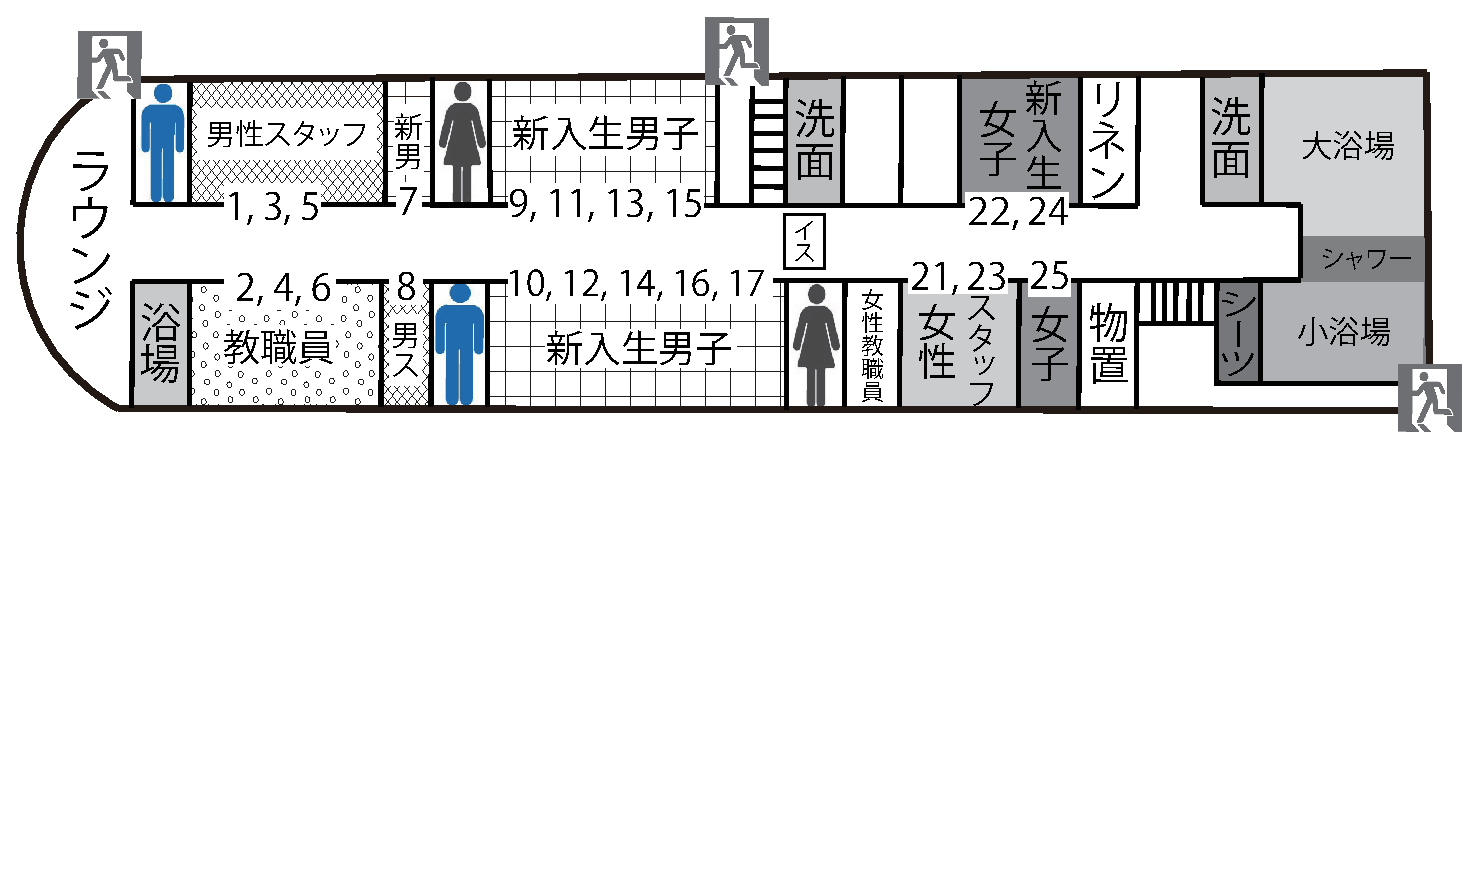
\includegraphics[scale=0.6]{./10/syushin.eps}
\vspace{-45mm}
\caption{就寝部屋割り}
\label{fig:futon_katazuke}
\end{center}
\end{figure}

\subsection{スタッフの就寝部屋}
\begin{figure}[H]
\begin{center}
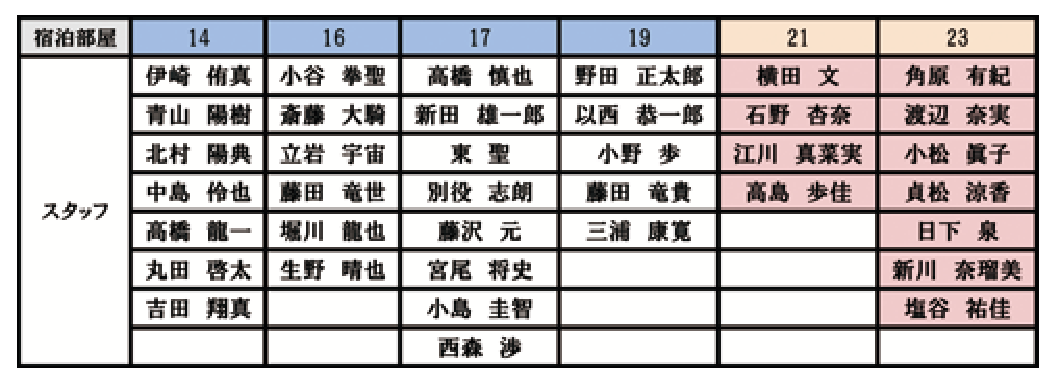
\includegraphics[scale=0.9]{./10/room.eps}
\end{center}
\end{figure}

% 注意事項やスタッフに周知しておくべきことがあれば記入する
\subsection{備考}
\begin{itemize}
%\item 小松(くろしお棟1担当スタッフ),宮尾(くろしお棟3担当スタッフ)は野外炊事から荷物を取りに行く時,第一集会室にいる岡本から指導者棟(龍馬・慎太郎)の鍵をもらう
%\item 基本的に,小松,宮尾が指導者棟の鍵を岡本に返却するまで,スタッフは指導者棟を使用しない
%\item その他,指導者棟の鍵が必要な人は鍵係(岡本)に連絡して鍵をもらう(指導者棟を利用する場合は,適宜報告LINEに連絡する)
%\item 時間や手間の都合上鍵を又貸しする場合は,その旨を報告LINEに報告して誰が鍵をもっているのか明確にしておく
%\item 鍵係は常に連絡がとれる状況にしておく
\item 小松,小島,西森,堀川は、夜の宴終了間近に入浴しないようにする。
\end{itemize}

% \subsection{連絡事項}
% \begin{table}[h]
% \begin{tabular}{|c|c|c|c|}
% \hline
% {報告者}&{内容}&{タイミング}&{備考}\\ \hline\hline
% Aさん & 指導者棟・慎太郎の浴場使用 & 1回目入浴開始時 & 大浴場で入浴できない新入生がいた場合のみ\\ \hline
% Bさん & 指導者棟・龍馬の浴場使用 & 1回目入浴開始時 & 小浴場で入浴できない新入生がいた場合のみ\\ \hline
% Cさん & くろしお棟1の入浴終了 & 1回目入浴終了時 & \\ \hline
% Dさん & くろしお棟3の入浴終了 & 1回目入浴終了時 & \\ \hline
% Fさん & 指導者棟・慎太郎の浴場使用 & 2回目入浴開始時 & 大浴場で入浴できない新入生がいた場合のみ\\ \hline
% Gさん & くろしお棟2の入浴終了 & 2回目入浴終了時 & \\ \hline
% \end{tabular}
% \label{tab:bath}
% \caption{各棟入浴開始時間}
%\end{table}

%\include{end}
